% command to make sure colorboxes don't create whitespace between code lines
\fboxsep=.6pt

% default settings for listings
\lstset{style=TigerJython, basicstyle=\scriptsize\ttfamily}

\begin{frame}
	\centering
	\begin{figure}[H]
		
\includegraphics[keepaspectratio, width=0.7\paperwidth, height=\paperheight]{LeeLogo}
	\end{figure}
	Informatik: Programmieren\\
	\emoji{clipboard} Kapitel 5: \textbf{Listen} (Bubble Sort)
\end{frame}

\newcommand{\includesteps}[1]{%
	\foreach \step in {1,...,#1}{%
		\only<\step>{%
			\begin{figure}[H]
				\input{GrundlagenInfo/00_Programmieren/Python/step_\step.tex}
			\end{figure}
		}%
	}
}

\begin{frame}[fragile]{Sortier-Algorithmen}
Wie kommen wir von \lstinline|x = [5, 3, 8, 20, 2, 10]|	zu \lstinline|x = [2, 3, 5, 8, 10, 20]|?
\begin{itemize}[<+->]
	\item \textbf{Algorithmus} = \textit{eindeutige} und \textit{endliche} Abfolge von Anweisungen oder Schritten zur Lösung eines Problems
	\item \textbf{Sortieren}: Wichtig, um Daten zu organisieren, Zugriff und die Suche nach Elementen effizienter zu machen und bildet die Grundlage für viele weitere Anwendungen und Algorithmen (z.B. \textit{Suche}).
	\begin{figure}[H]
			\centering
			\raisebox{-0.5\height}{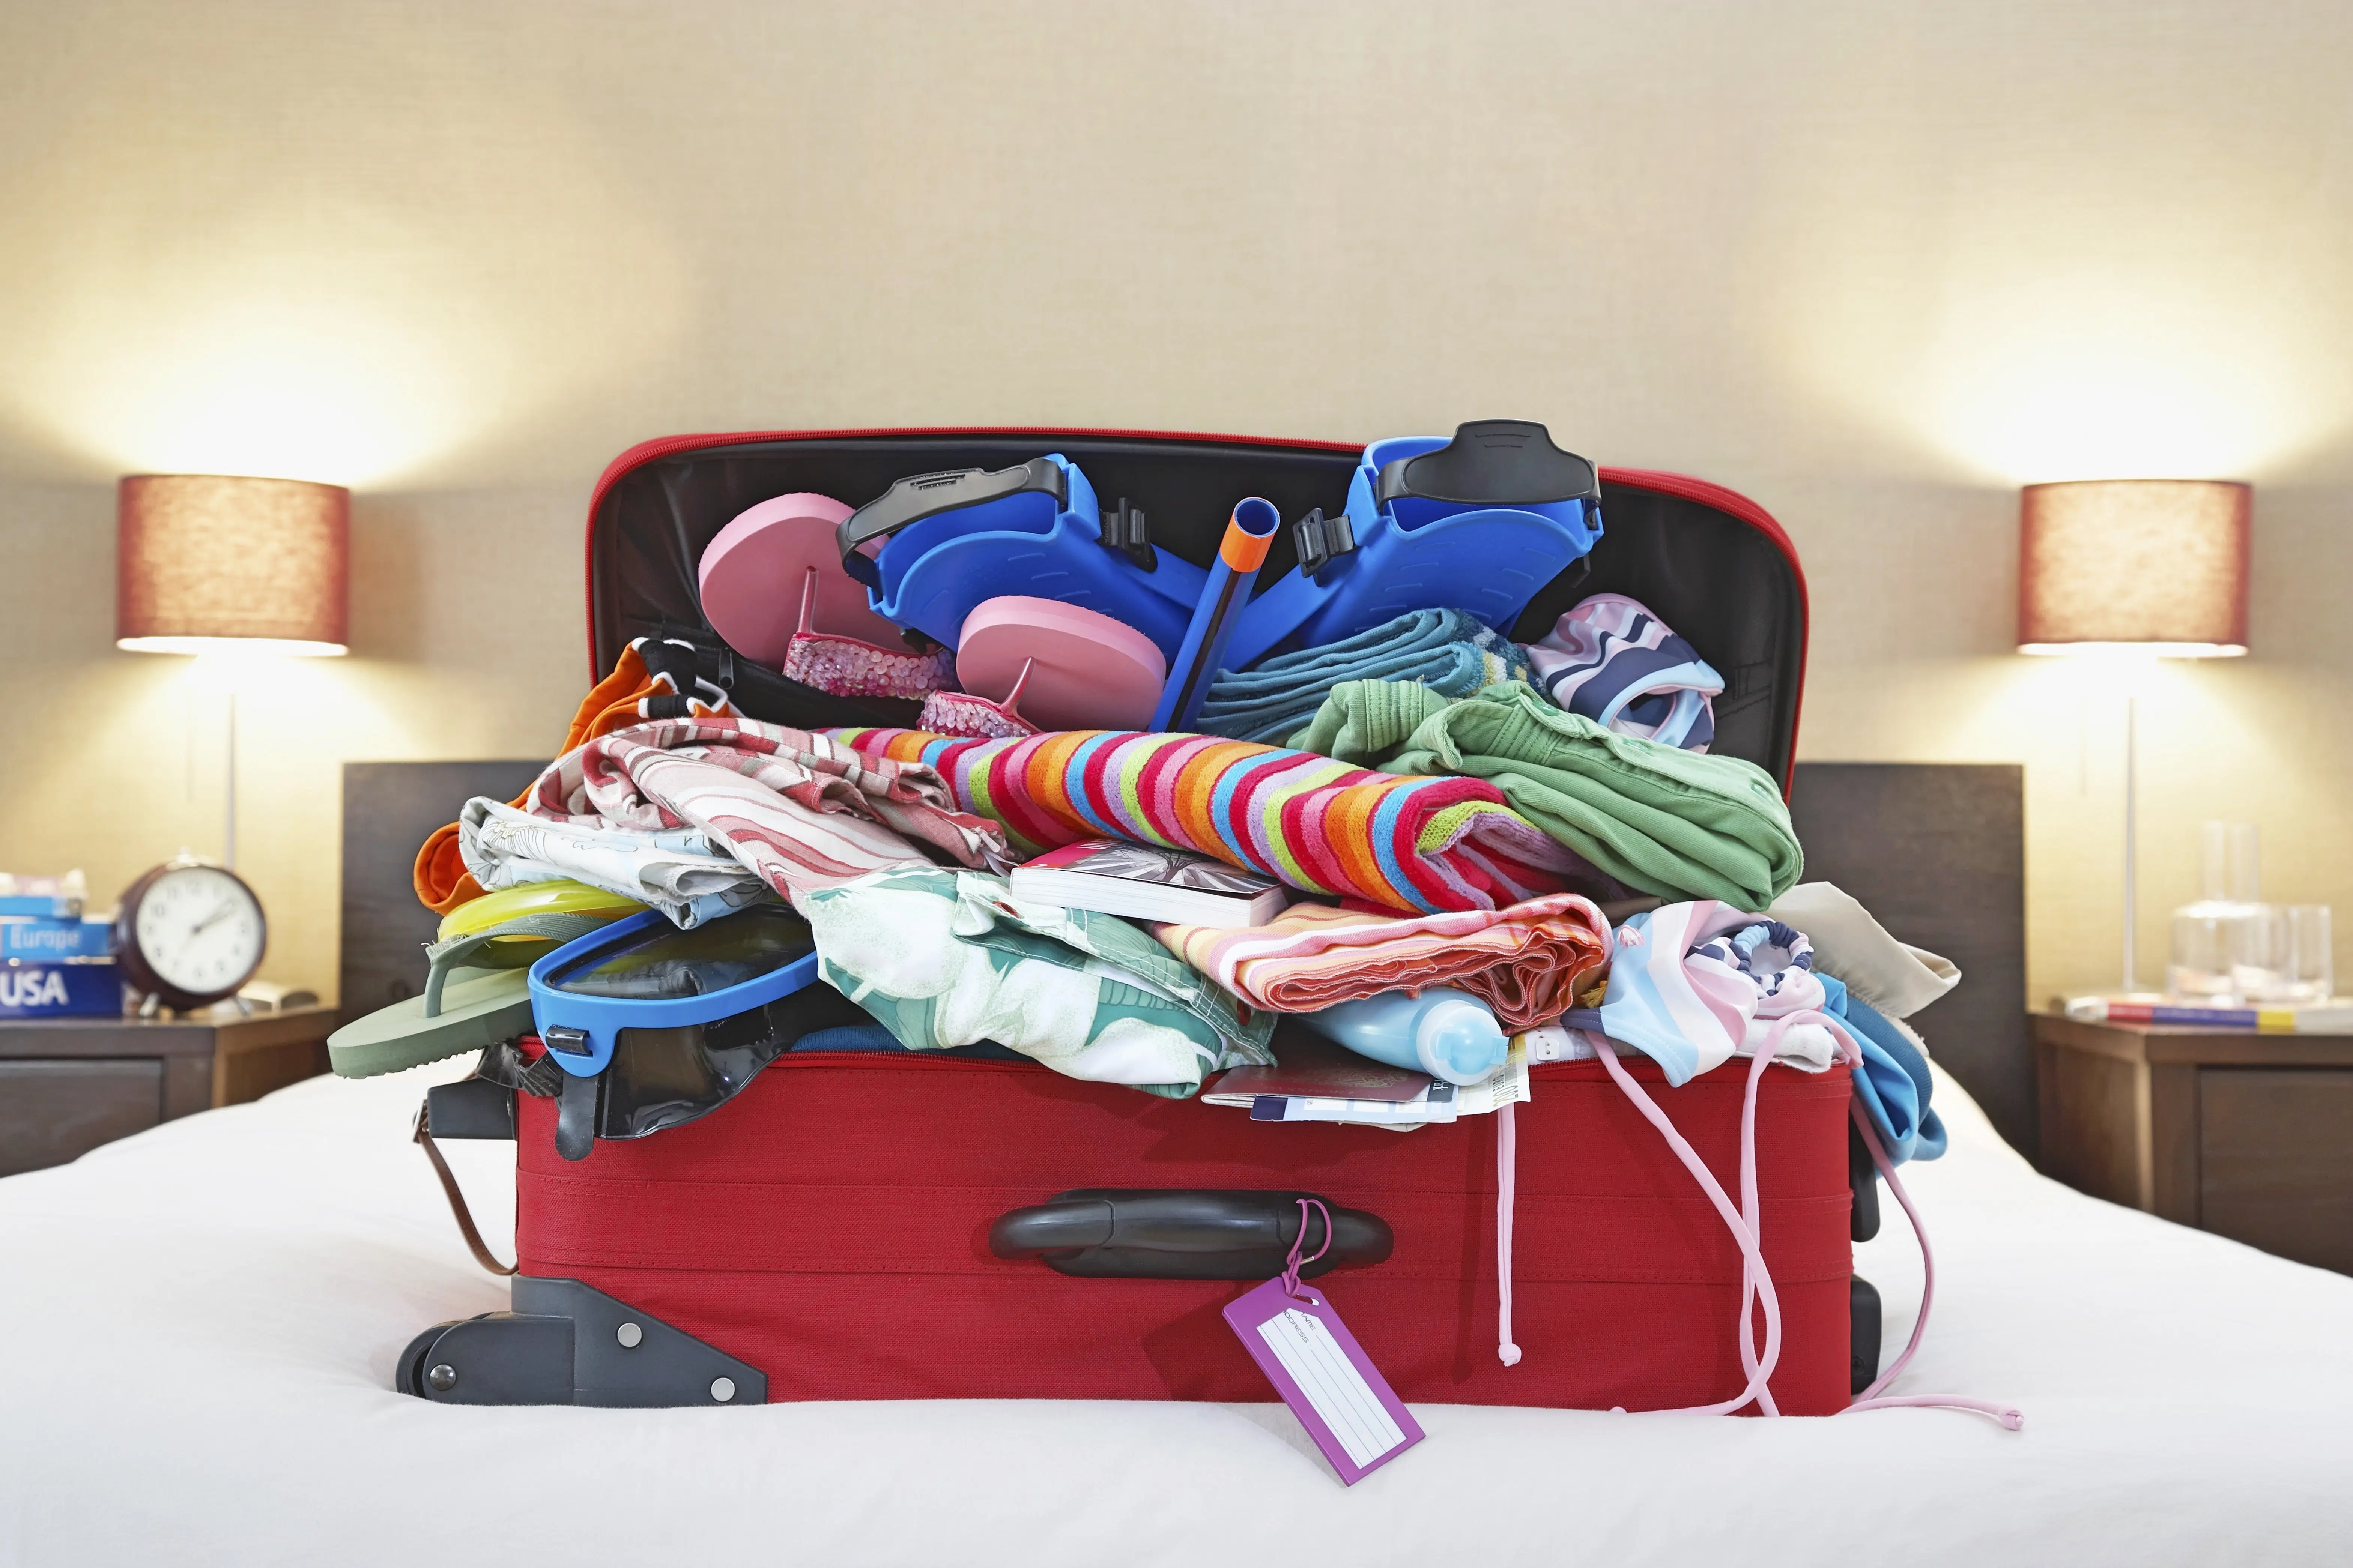
\includegraphics[width=.3\textwidth]{GrundlagenInfo/04_Kompression/Figures/messy_suitcase.jpg}}
			\raisebox{-0.5\height}{$\rightarrow$}
			\raisebox{-0.5\height}{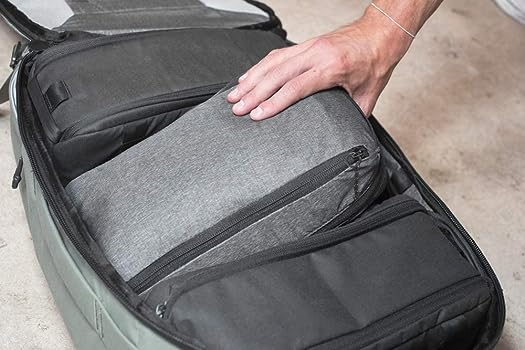
\includegraphics[width=.3\textwidth]{GrundlagenInfo/00_Programmieren/Figures/prog-packing-cubes}}
		\end{figure}
\end{itemize}
	
\only<3->{Heute: \textbf{Bubble-Sort-Algorithmus}}
\end{frame}

% Replace <number_of_steps>tete with the actual number of steps generated
\begin{frame}[fragile]{Bubble-Sort-Algorithmus}{Visualisierung}
	\includesteps{21}
\end{frame}

\begin{frame}[fragile]{Bubble-Sort-Algorithmus}{Python-Code}
	\begin{lstlisting}
# x ist die Liste, die sortiert werden soll
x = [5, 3, 8, 20, 2, 10]

# Äussere Schleife
repeat len(x) - 1:
    index = 0
    # Innere Schleife: Vergleiche benachbarte Elemente
    repeat len(x) - 1:
    	# Tausch von x[index] und x[index + 1], falls falsche Reihenfolge
        if x[index] > x[index + 1]:
            z = x [index]
            x[index] = x[index + 1]
            x[index + 1] = z
         
        index += 1
    print(x)
	\end{lstlisting}

\end{frame}

\begin{frame}[fragile]{Laufzeit des Algorithmus}
Anzahl Vergleiche, falls die Liste $n$ lang ist
\begin{itemize}[<+->]
	\item Allgemein
	\begin{itemize}
	\item Nicht optimierte Version: 
	\[(n-1)^2\]
	\item Optimierte Version:
	\[\sum_{m=1}^{n-1}m \]
	\end{itemize}
	\item Also z.B., falls Liste 6 Elemente enthält
	\begin{itemize}
	\item Nicht optimierte Version: $(5)^2=25$ Vergleiche
	\item Optimierte Version: $\sum_{m=1}^{5}m = 15$ Vergleiche
	\end{itemize}
\end{itemize}
\end{frame}


\begin{frame}[fragile]{Auftrag}
\begin{itemize}
\item Schauen Sie sich den Python-Code für Bubble Sort auf Moodle an sowie die folgenden drei Listen:
\begin{itemize}
\item \lstinline|x = [3, 4, 1, -3, 6]|
\item \lstinline|x = [3, 4, 5, 6, 7]|
\item \lstinline|x = [7, 6, 5, 4, 3]|
\end{itemize}
Notieren Sie von Hand, wie die Listen nach jedem Durchgang der äusseren Schleife aussehen (für eine Liste von Länge 5 sollten Sie beispielsweise 4 Zwischenresultate notieren). Kontrollieren Sie Ihr Resultat, indem Sie das Programm mit diesen Listen ausführen.
\item \challengebox{Aufgabe 5.12}
\end{itemize}
\end{frame}

